%Das ist die Hauptdatei. 
%Diese Datei ist die, welche von pdflatex übersetzt wird (erzeugt dann pdf). 
%Dieses Liederbuch nutzt das Latex Songs Package, welches unter der GPLv2 steht. 
%Eine Kopie der GPLv2 kann hier eingesehen werden: https://opensource.org/licenses/gpl-2.0.php 
%Kurzum sagt die Lizenz, dass das Paket genutzt werden darf, und dass der Entwickler des Paketes 
%für nichts haftbar gemacht werden kann. 
%Durch die Nutzung des Paketes steht dieses Liederbuch automatisch auch unter der GPLv2 Lizenz. 
%Für uns heißt das, wenn wir nach Quellcode gefragt werden, diesen auch ausgeben müssen. 
%Wer unser Liederbuch modifiziert, muss bei Nachfrage ebenfalls sein Buch offenlegen. 
%Es muss kenntlich sein, dass Nutzer des Liederbuches diese Rechte haben, 
%somit muss (am besten in diesem Buch selbst) auf die Lizenz hingewiesen werden. 
%Ein entsprechender Verweis wurde auf der Titelseite angebracht. 
%Ein weiteres Problem stellt das Urheberrecht dar, wenn man ein solches Liederbuch bastelt. 
%Tatsächlich ist es so, dass wir den gesamten Quellcode rausrücken müssen, wenn wir gefragt werden. 
%Wir dürfen aber die vom Urheberrecht geschützen Liedtexte nicht einfach öffentlich zum Download anbieten. 
%Mein Ansatz hierfür wäre, die Lieder als separates Projekt anzusehen und auch so zu pflegen,
%denn dann trifft die GPLv2 nicht auf die Lieder sondern nur auf das Master-Layout zu. 
%Die offizielle Version des letzten Satzes ist dann: "Wir nutzen nur Urheberrechtlich ungeschütztes Material 
%und solches, von welchem wir eine Genehmigung haben"

\documentclass{book}
\usepackage[lmargin=10mm, rmargin=5mm, tmargin=2mm, bmargin=2mm, text={15cm,10cm},centering]{geometry}
\geometry{papersize={148mm,105mm}}
\usepackage[bookmarks]{hyperref}
\usepackage[chorded]{songs}
\usepackage{graphicx}
\usepackage[ngerman]{babel}

\pagestyle{empty}

\newindex{titleidx}{cbtitle}
\newauthorindex{authidx}{cbauth}
\newscripindex{scripidx}{cbscrip}

\songcolumns{1}
\usepackage[parfill]{parskip}
\renewcommand{\lyricfont}{\sffamily\small}
\renewcommand\printchord[1]{\sffamily\textmd\large#1}
\renewcommand{\stitlefont}{\sffamily\textmd}
\versesep=8pt

\begin{document}
\begin{titlepage}
\vspace*{\stretch{1.0}}
\begin{center}
{\sffamily\huge\bfseries Klampfenkrampf\par}
{\sffamily\small\bfseries Liederbuch\par}
\vspace{0.5cm}
{\sffamily\Large DPSG Neckarelz-Diedesheim\par}
\vspace{0.5cm}
{\sffamily\Large Stamm Don Bosco\par}
\vspace{0.5cm}
\begin{figure}[h]
\centering

\includegraphics[width=0.4\textwidth]{img/logo.jpg}\par\
\end{figure}
{\sffamily\small Zuletzt am \today{} aktualisiert\par}
\vspace{0.5cm}
{\sffamily\tiny Das Layout dieses Buches steht unter der Gnu General Public License Version 2.0.\par}
\end{center}
\vspace*{\stretch{2.0}}
\end{titlepage}


\begin{songs}{titleidx,authidx,scripidx} 
	\beginsong{Der Lagerboogie}[by={}]
\beginverse
Wir \[E]laden Sie zum Boogie ein, dann bleiben Sie auch \[B7]fit. Wir singen eine Strophe vor und dann singt jeder \[E]mit.
\endverse

\beginchorus
Ja ja ja, tschu tschu, der Lagerboogie ist unser \[B7]Boogie-Woogie, tschu tschu tschu, die Zeit vergeht im \[E]Nu.
\endchorus

\beginverse
Und \[E]eins und zwei und drei und vier, und drei und zwei und \[B7]eins, der Text der ist ganz Schnuppe hier, die Hauptsache es \[E]reimt.
\endverse

\beginverse
Der \[E]Text kann noch viel dümmer sein, das macht uns gar nichts \[B7]aus, wir stimmen in das Liedchen ein und brüllen voll he\[E]raus.
\endverse

\beginverse
Der \[E]Adam sang den Boogie schon, den Boogie singen \[B7]wir. Der Boogie ist der beste Song, drum eins, zwei, drei und \[E]vier. 
\endverse

\beginverse
Im \[E]Pfarrhaus ist ein großer Krach, Herrn Pfarrer hört man \[B7]schon, denn jeden Morgen um halb acht, da singt er diesen \[E]Song.
\endverse

\beginverse
Die \[E]Kuh gibt Süß- und Sauermilch den lieben langen \[B7]Tag. Der Ochse dieses dumme Vieh gibt leider nur Spi\[E]nat.
\endverse

\beginverse
Es \[E]schreit die Geiß, es bellt der Hund, die Kuh brüllt dazu \[B7]muh, dem Vogel ist's schon lang zu bunt, er will jetzt seine \[E]Ruh'.
\endverse

\beginverse
Vom \[E]Boogie wackelt schon die Wand, die Scheiben fallen \[B7]aus und doch sind wir jetzt noch nicht still und singen voll he\[E]raus. 
\endverse

\beginverse
Wir \[E]haben nun genug geseh'n und wollen jetzt nach \[B7]Haus, wir wollen jetzt nach Hause geh'n so lasst und endlich \[E]raus. 
\endverse

\beginverse
Die \[E]kleine Möve Jonathan, die regt mich ganz schön \[B7]auf, drum nehm ich ihren Kopf und hau' ein paarmal feste \[E]drauf!
\endverse

\beginchorus
Ja ja ja, tschu tschu, der Lagerboogie ist unser \[B7]Boogie-Woogie, tschu tschu tschu, die Zeit vergeht im \[E]Nu.
\endchorus

\vspace{10mm}

\rule{\textwidth}{0.5pt}

\vspace{2.5mm}

\rule{\textwidth}{0.5pt}

\vspace{2.5mm}

\rule{\textwidth}{0.5pt}

\vspace{2.5mm}

\rule{\textwidth}{0.5pt}

\newpage

\mbox{}

\vfill

\centering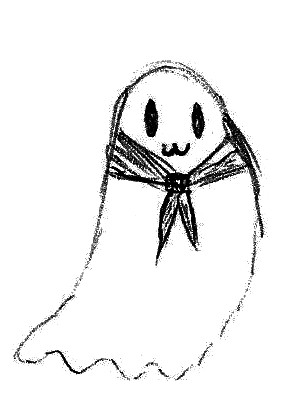
\includegraphics[width=4cm]{img/lagerboogie.jpg}

\vspace*{\fill}

\endsong

\beginsong{Grifftabellen}[by={}]
\gtab{A}{X02220} \gtab{A7}{X02020} \gtab{Am}{X02210} \gtab{Am7}{X02010} \gtab{Am/G}{302210} \gtab{Am7/G}{302010}
\gtab{A#}{X(13331)} \gtab{A#dim}{X12320}
\vspace{0mm}

\gtab{B}{2:X(13331)} \gtab{B7}{X21202} \gtab{Bm}{2:X(13321)} \gtab{Bm7}{X20202}
\vspace{0mm}

\gtab{C}{X32010} \gtab{C7}{X32310} \gtab{Cadd9}{X32033} \gtab{C/B}{X22010} \gtab{C/E}{032010} \gtab{C/G}{332010} \gtab{Cm}{3:X(13321)} \gtab{Cm7}{3:X(13121)}
\vspace{0mm}

\gtab{D}{XX0232} \gtab{D7}{XX0323} \gtab{Dsus4}{XX0233} \gtab{D/F#}{2X0200} \gtab{D7/F#}{23021X} \gtab{Dm}{XX0231} \gtab{Dm6}{XX0201} \gtab{Dm7}{XX0211} \gtab{Dm/F}{XX3231}
\vspace{0mm}

\gtab{E}{022100} \gtab{E7}{022130} \gtab{E7sus4}{020200} \gtab{Em}{022000} \gtab{Em7}{022030}
\vspace{0mm}

\gtab{F}{(133211)} \gtab{F6}{(113211)} \gtab{F7}{(131211)} \gtab{Fm}{(133111)} \gtab{Fm7}{(131111)}
\gtab{F#m}{2:(133111)} \gtab{F#m7}{202220}
\vspace{0mm}

\gtab{G}{320033} \gtab{Gsus4}{3:(113311)} \gtab{G6}{320000} \gtab{G7}{320001} \gtab{G/B}{X2003X} \gtab{Gm}{3:(133111)} \gtab{Gm7}{3:(131111)}
\vspace{0mm}

\vspace{\fill}

\endsong


\end{songs}

\showindex{Inhaltsverzeichnis}{titleidx}
%nicht genutzte indizes für andere inhaltsverzeichnisse
%sollen diese genutzt werden, muss das makefile angepasst werden!
%\showindex{Index of Authors and Composers}{authidx}
%\showindex{Index of Scripture}{scripidx}

\end{document}

